\documentclass[13pt]{beamer}
\usetheme{Frankfurt}
\usecolortheme{beaver}

\usepackage[spanish]{babel}
\usepackage{amsmath}
\usepackage{amsfonts}
\usepackage{amssymb}
\usepackage{color}
\usepackage{xcolor}
\usepackage{listings}
\usepackage{graphicx}
\usepackage{wrapfig}

\definecolor{codegreen}{rgb}{0,0.6,0}
\definecolor{codegray}{rgb}{0.5,0.5,0.5}
\definecolor{codepurple}{rgb}{0.58,0,0.82}
\definecolor{backcolour}{rgb}{0.95,0.95,0.92}

\lstdefinestyle{mystyle}{
    basicstyle=\tiny,
    commentstyle=\color{codegreen},
    keywordstyle=\color{magenta},
    numberstyle=\tiny\color{codegray},
    stringstyle=\color{codepurple},
    basicstyle=\ttfamily\footnotesize,
    breakatwhitespace=false,         
    breaklines=true,                 
    captionpos=b,                    
    keepspaces=true,                 
    numbers=left,                    
    numbersep=5pt,                  
    showspaces=false,                
    showstringspaces=false,
    showtabs=false,                  
    tabsize=2,
	xleftmargin=8pt
}

\lstset{style=mystyle, basicstyle=\scriptsize}

\author{Shao Jie Hu Chen \and Mario Megías Mateo \and Jesús Samuel García Carballo}
\title{Práctica 2. Divide y Vencerás}
\subtitle{Algorítmica}
%\logo{
\includegraphics[scale=0.05]{logo-ugr.jpeg}}
\institute{Equipo Rojo}
%\date{}
%\subject{}
%\setbeamercovered{transparent}
\setbeamertemplate{navigation symbols}{}

\begin{document}
	
	\begin{frame}[plain]
		\maketitle
		% \begin{center}
		% 	
\includegraphics[scale=0.15]{logo-ugr.jpeg}
		% \end{center}
	\end{frame}
	
	\begin{frame}
		\frametitle{Índice de contenidos}
		\tableofcontents
	\end{frame}

    % Introducción

    \section{Introducción}

    \begin{frame}
        \frametitle{Objetivos y motivación}

        \begin{itemize}
            \item \textbf{Implementar} algoritmo de tipo Divide y Vencerás.
            \item \textbf{Saber reconocer} el alcance y las limitaciones de algoritmos 
            de tipo Divide y Vencerás en ejemplos particulares.
        \end{itemize}

    \end{frame}

    \begin{frame}
        \frametitle{Metodología}

        \begin{figure}[h]
            \centering
            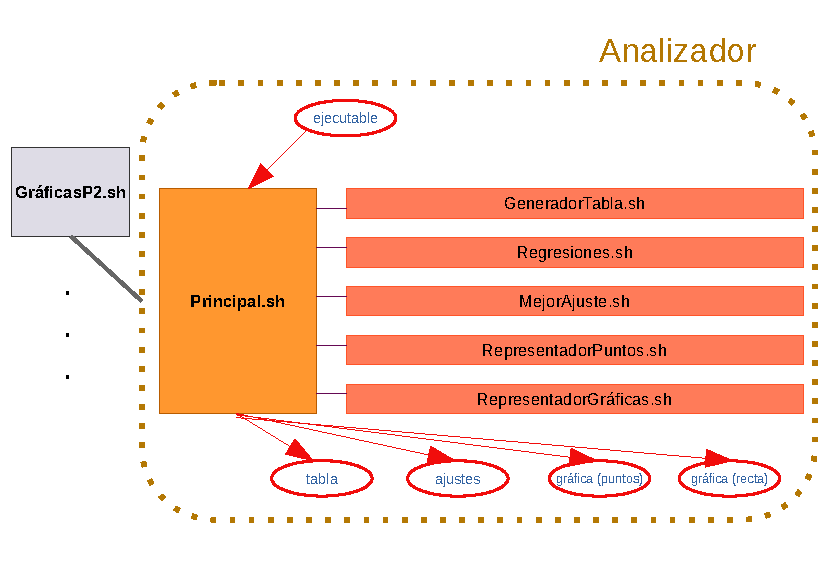
\includegraphics[scale=0.65]{img/esquema_graphkiller.pdf}
            \caption{Esquema de funcionamiento del \textbf{Analizador} \cite{Rojo2022}. Elaboración propia.}
            \label{fig:analizador}
        \end{figure}
    \end{frame}

    \begin{frame}
        \frametitle{Equipo empleado}

        \begin{block}{Especificaciones técnicas del equipo}
            \begin{itemize}
                \item \textbf{Procesador}: Intel(R) Core(TM) i7-9750H CPU @ 2.60GHz
                \item \textbf{Memoria RAM:} 32 GB DDR4
                \item \textbf{Sistema Operativo}: Ubuntu 20.04.4 LTS
            \end{itemize}
        \end{block}
    \end{frame}


    % Ejercicio 1

    \section{}


    \section{Ejercicio 1b}

    \begin{frame}
        \frametitle{Descripción}
        \begin{block}{Problema}
            Dado un vector de n componentes ordenado de menor a mayor (con \textbf{valores repetidos}), 
            encontrar $i$ tal que $v[i] = i$. 
        \end{block}

        \begin{alertblock}{Fallo del algoritmo anterior}
            El algoritmo propuesto para el caso con valores no repetidos \textbf{no es válido}.
        \end{alertblock}
    \end{frame}

    \begin{frame}
        \frametitle{Ejemplo de funcionamiento erróneo}
        \begin{figure}
            \centering
            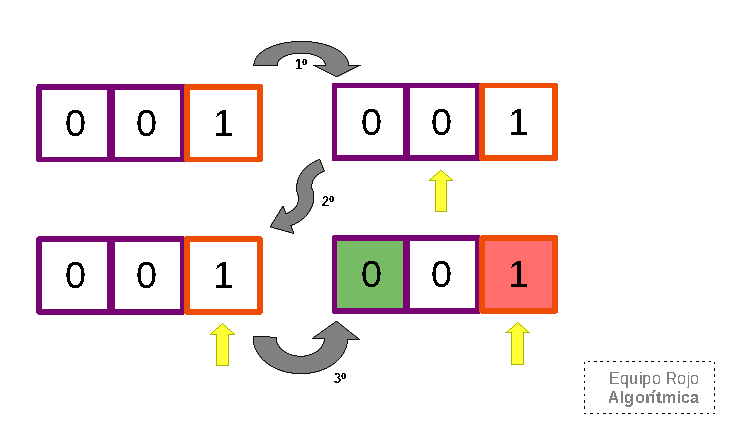
\includegraphics[scale=0.81]{img/esquema_fallo1a.pdf}
            \caption{Vector con elementos repetidos para el que falla 
            el algoritmo anterior. Elaboración propia.}
            \label{fig:fallo-1a}
        \end{figure}
    \end{frame}

    \begin{frame}
        \frametitle{Modificación del algoritmo}

        \lstinputlisting[caption=Pseudocódigo asociado al caso Divide y Vencerás., label={alg:1b-dyv}]{listing/ejer1b-pseudo-dyv.txt}
    \end{frame}

    \begin{frame}
        \begin{exampleblock}{Implementación en C++}
            \lstinputlisting[language=C++, firstline=114, lastline=134, label={cod:1b-dyv}]
            {../src/ejercicio-1-comp-fija-repetidos.cpp} 
        \end{exampleblock}
    \end{frame}

    \begin{frame}
        \frametitle{Análisis de Eficiencia}

        \begin{block}{Ecuación en diferencias asociada}
            \begin{equation}
                T(n) = \left\{ \begin{array}{lr} 2 T(n/2) + c & \text{si } n > \text{UMBRAL}\\ n & \text{si } n \leqslant \text{UMBRAL} \end{array} \right.
                \label{eq:1b-efi-dyv-rec}
            \end{equation}

            Por tanto:

            \begin{equation*}
                \boxed{T(n) \in O(n)}
            \end{equation*}
        \end{block}
        
    \end{frame}

    % Ejercicio 2

    % Conclusiones

    % Bibliografía

    \section{Bibliografía}

    \begin{frame}
        \begin{thebibliography}{0}
            \bibitem{Verdegay2017} Verdegay Galdeano. (2017). Lecciones de Algorítmica / José Luis Verdegay. Técnica Avicam.
            \bibitem{Cormen2017} Cormen. (2017). Introduction to algorithms / Thomas H. Cormen... [et al.] (3rd ed.). PHI Learning.
            \bibitem{Garrido2018} Garrido Carrillo. (2018). Estructuras de datos avanzadas: con soluciones en C++ / A. Garrido. Universidad de Granada.        
            \bibitem{Rojo2022} Hu Chen. (2022). Práctica 1: Análisis de Eficiencia de Algoritmos / Shao Jie Hu, J. Samuel García y Mario Megías.      
        \end{thebibliography}
    \end{frame}

\end{document}